\documentclass[oneside]{book}
\usepackage{amssymb,latexsym,color,amsthm,parskip,hyperref}

%allows for comment blocks and verbatim sections
\usepackage{verbatim}

%preserves tabs in verbatim sections. Good for including source code in documents.
\usepackage{moreverb}

%The following are for the example boxes
\usepackage{graphicx}
\definecolor{Dark}{gray}{.20}
\definecolor{Light}{gray}{.80}
\newcommand{\examplein}[1]{\begin{center} \colorbox{Dark}{\textcolor{white}{#1}} \end{center}}
\newcommand{\exampleout}[1]{\begin{center} \colorbox{Light}{\textcolor{black}{#1}} \end{center}}

\usepackage{listings,color,xcolor}
\definecolor{verbgray}{gray}{0.9}


\lstnewenvironment{code}{
    \lstset{backgroundcolor=\color{verbgray}, 
    frame=single,
    framerule=0pt,
    basicstyle=\ttfamily,
    columns=fullflexible}}{}

\lstnewenvironment{gitcode}{
    \lstset{backgroundcolor=\color{cyan!10}, 
    frame=single,
    framerule=0pt,
    basicstyle=\ttfamily,
    columns=fullflexible}}{}
    
\lstnewenvironment{svncode}{
    \lstset{backgroundcolor=\color{red!10}, 
    frame=single,
    framerule=0pt,
    basicstyle=\ttfamily,
    columns=fullflexible}}{}

\begin{document}

\title{Understanding Version Control}
\author{Kendra De Groot, Andy Brown, and Robin Cosbey}

\maketitle
\tableofcontents
\newpage
\chapter{Introduction}
%Kendra
% General concepts for version control use
\section{Why Version Control is Awesome}
Think about your last programming project and all the hours you put into it. If you lost progress on the project what would you do? What if you wanted to go back to a previous way you had the program written? Using version control saves you from accidentally deleting your files and allows you to switch between versions with ease.\\

Version control also allows every member of a team to work on any file in a project at the same time. When you're done, you can merge your changes to a shared repository that is assured to have the latest version of the file. You could also easily work from home by cloning your files through an SSH tunnel and save yourself from emailing or making copies of files on a USB drive. Version control will be incredibly helpful for any collaborative events, such as the spring Hackathon and quarterly Game Jams.

\section{Repositories and Working Directories}
A repository holds a set of commit objects and a set of references to those commit objects which are called heads.
The working directory is a version of a project that has been checked out to work on.
For Git, the repository is stored in the same directory as the project, in a .git sub-directory. SVN has a central-repository system instead and the repo isn't stored in files alongside the project.
\subsection{Repository Files, a cautionary tale}
Every guide on version control software will warn you not to edit the files in your repository directly. Only edit files and use commands in your working directory that will then get sent to your repository. It is possible to corrupt your repository by editing the files within it which can lead to lost work and time. If your repository is being accessed by more than one person there is even more danger of breaking things. In general use, there will be no need to touch anything directly within your repository. 
\\
\\

\begin{figure}[ht!]
	\centering
	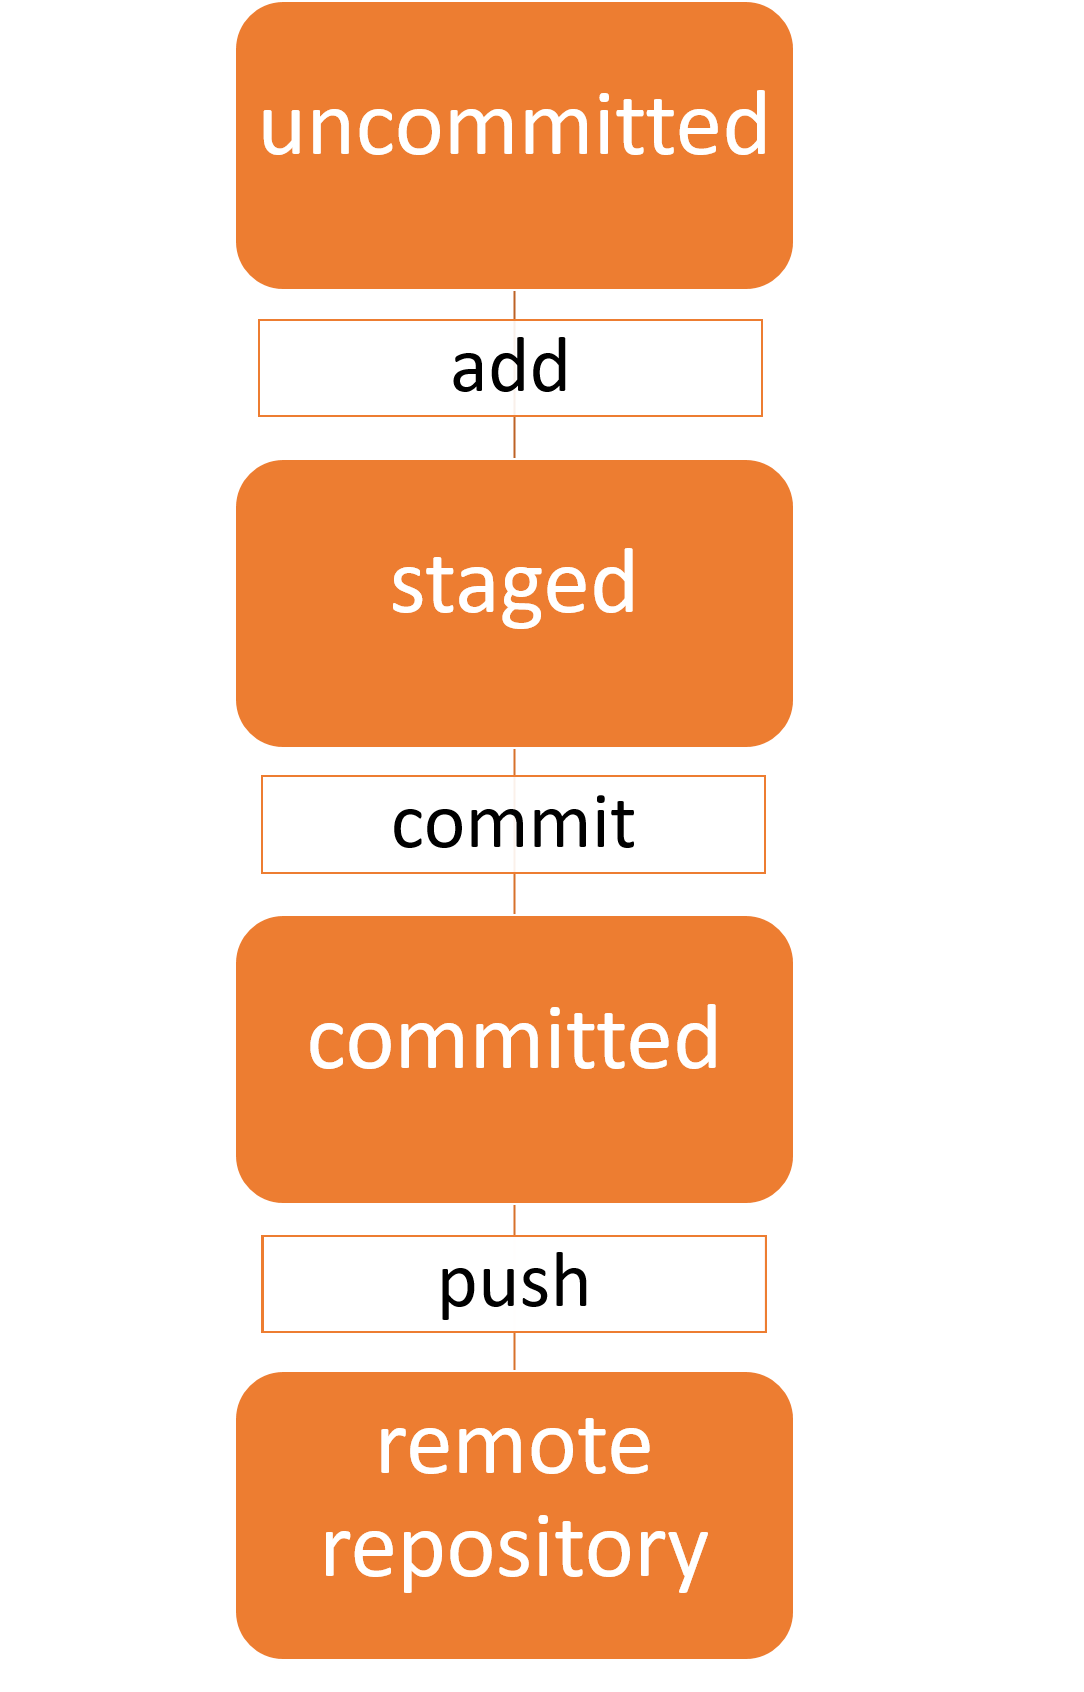
\includegraphics[width=70mm]{introduction.png}
	\caption{Stages of a file} 
\end{figure}


\chapter{Local Repositories}
We begin with all of the tools that you need to create and manage a repository on your local machine. Commands with a blue background correspond to git and commands with a pink background correspond to SVN. Text in commands with arrowheads around it signify required arguments that should be replaced with the desired value excluding the \textless \textgreater\  symbols. Text in commands with brackets around it signify optional arguments and should be replaced excluding the [ ] symbols.  
%Andy
\section{Initializing a Local Repository}
Both of these commands will create a new repository in the specified directory. The directory path is optional for git, as it will use your shell's current working directory when you do not specify a directory.
    \begin{gitcode}
    git init [directory]
    \end{gitcode}
    \begin{svncode}
    svnadmin create <directory>
    \end{svncode}
For git, you will now have a working directory with the repository files stored inside it in a .git folder. SVN requires you to create your own working directory. Be sure to use the absolute path to the repository to replace \textless repoDirectory\textgreater. If no working directory is supplied then SVN will use your shell's current working directory when checking out the repository.  

    \begin{svncode}
    svn checkout file:///<repoDirectory> [workingDirectory]
    \end{svncode}
    

%Robin
\newpage
\section{Basic Commands}
Listed below are some commands used frequently when managing a repository.\\ \\
\textbf{status} This command determines where the files are located in the repository. Calling status will show the user what files are untracked and any modifications that have been made to the working directory. In git, including the -s will give a simplified output which is generally used if there are a lot of files in the directory. 
    \begin{gitcode}
    git status
    git status -s
    \end{gitcode}
    \begin{svncode}
    svn st
    \end{svncode}
\textbf{add} Schedules a file to be added to the repository. When a file is added, it becomes a file that the repository tracks. You can also add a directory to the repository by including the directory name instead of a file name. In git, you will need to add each file that you wish to apply to each commit. You can use the -A flag to add \textbf{all} new, modified, and deleted files since your last commit. Likewise, the -u flag \textbf{updates} all modified and deleted files to be staged.\newline
In svn, once a file is added it is automatically tracked for future commits.
    \begin{gitcode}
    git add <file/directoryname>
    git add -A
    git add -u
    \end{gitcode}
    \begin{svncode}
    svn add <file/directoryname>
    \end{svncode}
\textbf{remove} Schedules a file or directory to be removed from the repository. 
    \begin{gitcode}
    git rm <file/directoryname>
    \end{gitcode}
    \begin{svncode}
    svn rm <file/directoryname>
    \end{svncode}
\textbf{move} Move a file to a different directory.
    \begin{gitcode}
    git mv <filename> <destinationname>
    \end{gitcode}
    \begin{svncode}
    svn mv <sourcename> <destinationname>
    \end{svncode}

\newpage
\section{Committing}
Committing a file records the changes in the repository. If the -m argument is supplied then the following string will be applied as the comment for the commit. Leaving off the -m argument will open up the default text editor to enter your commit comment.
    \begin{gitcode}
    git commit [-m `Comments here']
    \end{gitcode}
    \begin{svncode}
    svn ci [-m `Comments here']
    \end{svncode}
    
Suppose you accidentally made a spelling error in the commit message. If no files are currently staged, the \textbf{-{}-amend} flag allows you modify the previous commit's message without altering its snapshot. 

    \begin{gitcode}
    git commit --amend -m `new commit message'
    \end{gitcode}

\textbf{NOTE:} If there are files currently staged (i.e. you just ran the `git add' command), amending does not just alter the most recent commit, it replaces it entirely with a new commit. This may be okay for minor fixes on a personal project, but if you are working with other developers this could potentially cause a \hyperref[sec:conflict-resolution]{merge conflict!}
    
\subsection{Commenting}
It is important to include a descriptive comment about the changes you are committing. Ideally, you will be committing frequently, so you can simply write a description of what you changed in a function and why. If you use comments like ``updated code" or ``fixed bugs" you will have a hard time in the future if you ever need to look through the history of your project to pinpoint issues. This is also something that potential employers will look at when they ask to see a repository that you have worked on. Additionally, meaningful comments are exponentially more important when you are working with a team of people on the same project to stay coordinated with all changes. 

\subsection{Viewing the Commit History}
After a few commits you will have a running history of your project changes. To take a look at your history you can run the \textbf{log} command. This displays information about the commits made in your repository in reverse chronological order. Running the log command without any flags should produce output that looks like this:

\begin{figure}[ht!]
    \centering
	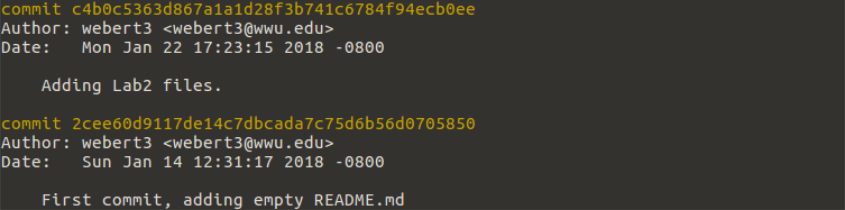
\includegraphics[width=120mm]{git_log_example.png}
	\caption{Typical output for `git log' command.} 
\end{figure}

By default the log command will display the commit's SHA-1 checksum (which you can think of as a unique identifier), as well as the name and email of the author (person who made the commit).

There are also several flags you can use to enhance the output of your log command. \textbf{-{}-stat} will show some abbreviated statistics for each commit, including the names of files changed, and the number of insertions/deletions made on each file. If you just want the commit id you can use the flag \textbf{-{}-pretty=oneline}. Your output would now look something like this:

\begin{figure}[ht!]
    \centering
	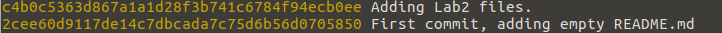
\includegraphics[width=120mm]{oneline.png}
\end{figure}

\subsection{Reverting Commits}
In git, \textbf{reset} unstages files that were previously added. This is a potentially dangerous operation as it cannot be undone and should not be used to undo commits that were pushed when sharing a repository. Applying the -{}-hard flag with  \textbf{reset} also changes the files in your working directory, overwriting any changes that you have made. If you wish to view the repository at a previous commit, you can use the \textbf{checkout} command to move to a specified commit. Checking out master will move you back to the latest commit. This is especially useful for individual files as the old versions that are checked out can then be committed. In svn, the \textbf{revert} command restores the version of the file or directory prior to any local modifications. You can use the \textbf{cat} command to view a file at a previous revision, and the \textbf{update} command can be used to update your current file to an older revision. 
    \begin{gitcode}
    git reset [--hard][HEAD~N]
    git checkout [HEAD~N / master] [file/directoryname] 
    \end{gitcode}
    \begin{svncode} 
    svn revert <file/directoryname>
    svn cat <-r N> file
    svn update <-r N> file
    \end{svncode}
Note: N refers to how far back to revert in git and revision number for svn.

\newpage
\section{Pushing and Pulling}
\textbf{Pulling} Your working directory is updated with the current contents of the associated repository. If you cloned a repository with git it will use that repository when pull is used with no repository specified. Likewise, the repository that you initially checked out with SVN will be the one that is used for updating. It's highly recommended to update your working directory before each session of working on your project. 
    \begin{gitcode}
    git pull [repository]
    \end{gitcode}
    \begin{svncode}
    svn update
    \end{svncode}
    
\textbf{Pushing} This sends your current commits to the origin or specified repository. Committing in SVN automatically applies your changes to the repository that is associated with your working folder.
    \begin{gitcode}
    git push [repository]
    \end{gitcode}
    
The first time you attempt to push a repository, you may get a message telling you that git.default is unset. There are two modes to choose from, matching and simple. If the default push mode is set to matching, then all of your local branches that share the same name as the remote repository will be updated on a push. When the mode is set to simple, then only the current branch that your repository would pull from would be pushed, assuming that their names match. It is recommended to use simple as it is more intuitive and can prevent potentially pushing to unintended branches. To set your push default to simple, use:
    \begin{gitcode}
    git config --global push.default simple
    \end{gitcode}
    

\newpage
\section{General Workflows}
\vspace{5mm}
\Large
General Git workflow looks like this:
\normalsize
\begin{enumerate}
    \item You pull from your repository to make sure you have up-to-date files.
    \item You write brilliant code in your working directory.
    \item You stage all files updated using add.
    \item You do a commit, which takes all the staged files and stores them in your Git directory.
    \item Repeat 2-4 as needed.
    \item You do a push which saves all of your commits to the repository. 
\end{enumerate}
\vspace{5mm}
\Large
General SVN workflow looks like this:
\normalsize
\begin{enumerate}
    \item You do an update to make sure you have up-to-date files.
    \item You write brilliant code in your working directory.
    \item You use add to stage any new files to track.
    \item You do a commit, which takes all the changed files and saves them to your SVN repository.
    \item Repeat 2-4 as needed.
\end{enumerate}
\vspace{5mm}
It's important to get in the habit of saving your project and documenting those changes.


\chapter{Branching}
%Kendra
\section{Why Branch?}
Branching is where you diverge from the main line of development and work in a new direction without using the main line. This allows you to try something new and go in a different direction with your code while still leaving your main project separate.

\begin{figure}[ht!]
    \centering
	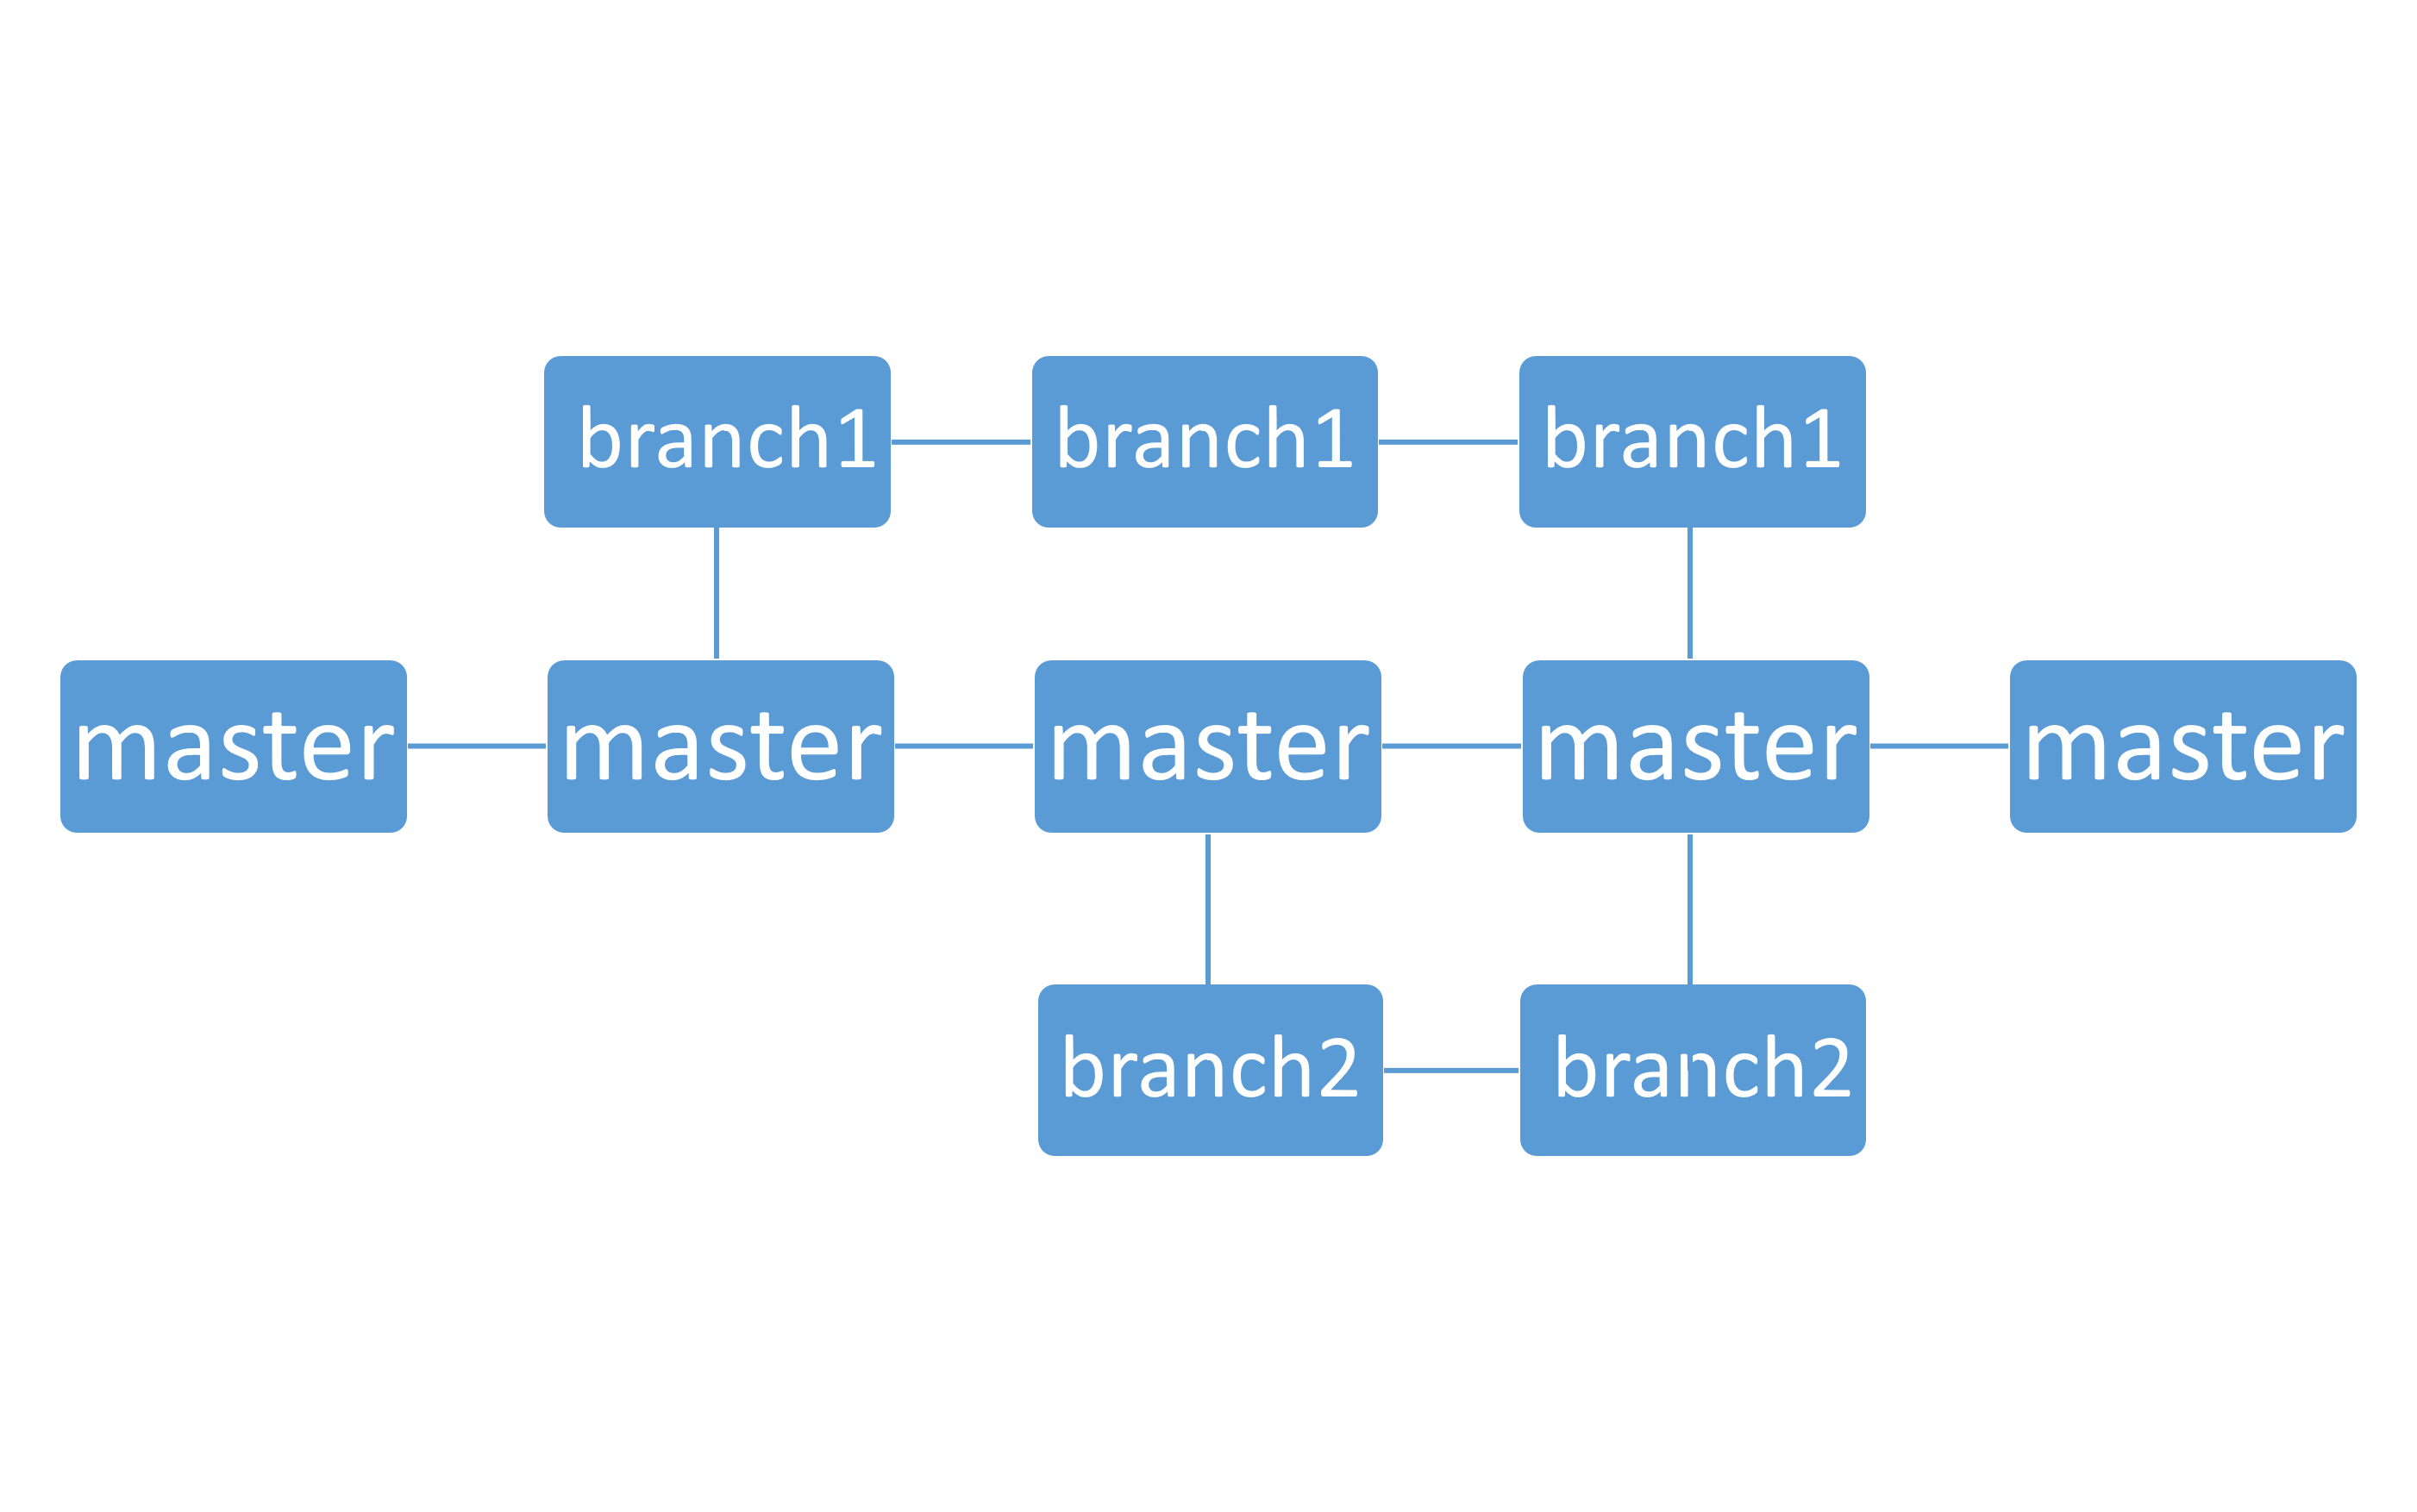
\includegraphics[width=120mm]{branching.png}
	\caption{An example of branching} 
\end{figure}

\section{Creating branches}
List all of the branches in your Git repo with:
    \begin{gitcode}
    git branch
    \end{gitcode}
Create a new branch named \textless branch-name\textgreater\ with:
    \begin{gitcode}
    git branch <branch-name>
    \end{gitcode}
Note: This only creates the branch, it doesn't check it out. To check out the branch \textless branch\textgreater\ use:
    \begin{gitcode}
    git checkout <branch-name>
    \end{gitcode}

For creating a branch using svn first you'll want to create a copy of your project tree in the repo using the svn copy command. For example say your current project is in/calc/trunk and you want to put it in a folder 'branches' under the name my-calc-branch, use:
    \begin{svncode}
    svn copy http://svn.example.com/repos/calc/trunk \
    http://svn.example.com/repos/calc/branches/my-calc-branch \
    -m "Creating a private branch of /calc/trunk."
    \end{svncode}

\section{Using Branches}
Branches are just pointers to commits. When you've finished a branch and have merged it into the main project, you can delete the branch without losing history.
To delete branch \textless branch-name\textgreater\ use:
    \begin{gitcode}
    git branch -d <branch-name>
    \end{gitcode}
Git won't let you delete the branch if it has unmerged changes, unless you use a capital D.
To merge your changes from a branch \textless branch-name\textgreater\ back into the branch you're in use:
    \begin{gitcode}
    git merge <branch-name>
    \end{gitcode}
If you want to merge your branches but always generate a merge commit use this:
    \begin{gitcode}
    git merge --no-ff <branch-name>
    \end{gitcode}
This is for documenting all the merges that occur in your repo.
\newline
\vspace{1mm}
\newline
For svn, in order to do a sync merge, where you bring your branch up-to-date before bringing its changes over to the new project use this when you are on your branch and where \textless url\textgreater\  is the URL for your main project:
    \begin{svncode}
    svn merge <url>
    \end{svncode}

    

\section{Tagging Revisions}
%tags and checkout of tagged revisions
Tagging is used to save a snapshot, for example a 1.0 or 2.0 version release to easily be restored to at a later time. In git, the process is a simple command that stores a pointer to the current commit. Conversely, in SVN you use the same procedure as branching, except targeting a folder you create named tags.
    \begin{gitcode}
    git tag -a <tagname> [-m <tagdescription>]
    \end{gitcode}
    \begin{svncode}
    svn copy http://svn.example.com/repos/calc/trunk \
           http://svn.example.com/repos/calc/tags/release-1.0 \
      -m "Tagging the 1.0 release of the 'calc' project."
    \end{svncode}
    
\chapter{Additional Topics}
    
\section{Conflict Resolution}
\label{sec:conflict-resolution}
%Andy
A merge conflict can occur when you try to update a file to the repository that has already been updated since the last time you updated your working directory. Merge conflicts are most common when working with other people on the same project, but they can easily happen if you forget to update your working directory before working on your project. 

While you can simply delete your changes and pull the most recent version of the file into your working directory to resolve the conflict, there are more elegant solutions that allow you to merge the work from both files available to both git and SVN.

For git, you begin your merge conflict by pulling from the remote repository. However, if you have unstaged changes to tracked files, you will not be able to pull from the remote repository. To fix this problem you can either commit the files or use the stash command to hide them away to be applied after the pull. All changes on tracked files will be reverted and stashed safely away.
    \begin{gitcode}
    git stash
    \end{gitcode}
    
Once you pull from the remote branch, you should apply your stashed files:
    \begin{gitcode}
    git stash apply
    \end{gitcode}
    
Now that you have pulled from the master branch, you should be ready to tackle the conflicted files. Performing a git status will show you any files that have conflicts, and git will automatically add both of the changes to the file with separators that show the range of the conflicts. Edit all of the files until the conflicts are resolved and add them to the staging area. Once your git status shows no more conflicting files, you are ready to update the changes. 

\newpage
There are generally two different cases that should be handled differently. If you had a previous commit before pulling, then you should perform a rebase to combine the pulled commits with your previous commit:
    \begin{gitcode}
    git rebase --continue
    \end{gitcode}

Otherwise, if you only stashed files before you pulled, you can create a new commit. Be careful not to commit if you already had a previous commit pending as it will cause additional steps to be required to complete the conflict resolution. Once you have rebased, or committed your stashed changes, you can then push the resolved files to the remote repository.
\smallskip \\

Furthermore, the resolution of conflicts can be made easier with different merge tools. You can setup a default merge tool in your git config, and then once you pull in a conflict you can use the merge tool to find and fix your conflicts. One commonly used merge tool is meld, which you can set as your default and then use as follows:

\begin{gitcode}
    git config --global merge.tool meld
    git mergetool
\end{gitcode}


    
    
\section{History}
%Kendra
\subsection{Diffs}
Git diff shows you the difference between versions of a file. To see the differences between your working directory and the index use:
    \begin{gitcode}
    git diff
    \end{gitcode}
Note: The index is synonymous with `cache' and `staged files'. It's the files you've staged for commit.
To see the difference between the index and the most recent commit use:
    \begin{gitcode}
    git diff -cached
    \end{gitcode}
To show the differences between your working directory and the most recent commit use:
    \begin{gitcode}
    git diff HEAD
    \end{gitcode}
For SVN, use:
    \begin{svncode}
    svn diff
    \end{svncode}
To show the local modifications in a working directory. You can also use:
    \begin{svncode}
    svn diff --old oldfile --new newfile
    \end{svncode}
Where oldfile and newfile are file names being compared. You can also specify the revision to examine by adding @this-revision after the file names where this-revision is the name of the revision to diff.
\subsection{Blame and Editing Commits}
To edit commits you can use:
    \begin{gitcode}
    git commit --amend
    \end{gitcode}
This will let you combine the staged changes you've made with the previous commit into one commit. It can also be used to just alter the commit message.
The blame command shows you who last modified each line of a file and when. To run the blame command on file with name \textless file-name\textgreater\ for git use:
    \begin{gitcode}
    git blame <file-name>
    \end{gitcode}



\section{Remote Repositories}
All of the concepts you have learned can now be applied to repositories that are not on your local machine. We begin this chapter with the basics of setting up SSH so you can tunnel to the linux cluster and directly access a repository from the school computers. We then look at other remote repository options. 
%Andy
\subsection{SSH Keys}
SSH (Secure Shell) keys provide a more secure method of establishing a connection than sending an encrypted password every time you connect. Once they are setup, a connection can be established without entering a password for every interaction.
\subsection{Creating Your Key}
Before creating your key, you may want to check and see if you've ever created a key in the past by entering:
    \begin{code}
    ls -al ~/.ssh
    \end{code}
To view your SSH directory. If you don't see the files:  \begin{verbatim}
    id_rsa and id_rsa.pub
\end{verbatim}
Then you can then generate them by entering:
    \begin{code}
    ssh-keygen -t rsa -b 4096 -C "<email address>"
    \end{code}
When asked to enter a file in which to save the key, just press Enter for the default location. You may enter a passphrase to be associated with your SSH key or optionally leave it blank by hitting enter. You should now see the two rsa files when you check your ssh folder as described above. 

\newpage
\subsection{Using Your Key}
Now that you have an SSH key, you will want to add it to the SSH agent to keep track of your passphrase. Make sure your SSH agent is running by entering:
    \begin{code}
    eval $(ssh-agent -s)
    \end{code}
    
You should get a result with an Agent pid. Assuming you created your key with the default directory and name, you can add your key to the ssh agent by entering:
    \begin{code}
    ssh-add ~/.ssh/id_rsa
    \end{code}
If you are at your home computer and wish to add your login to WWU to your SSH key, enter:
    \begin{code}
    ssh-copy-id username@linux.cs.wwu.edu -p 922
    \end{code}
Then enter your password, and now when you connect via ssh to the round-robin linux cluster you will use your SSH key for verification instead of typing in your school password every time. 
\subsection{Editing SSH Config}
Open up \texttt{\~}/.ssh/config with your favorite text editor. If you do not have a favorite you can enter: 
    \begin{code} 
    kate ~/.ssh/config 
    \end{code}
in the terminal to open up the file, then insert the following:
    \begin{code}
    Host wwussh
    HostName linux.cs.wwu.edu
    Port 922
    User WesternUsername
    \end{code}
Make sure you replace WesternUsername with your actual WWU username. Now you can use `ssh wwussh' to connect to the linux round-robin cluster instead of typing out the hostname and port. 

\newpage
\section{Tunneling To Your Repository}
Now that you went through all of that work, you can now easily check out repositories from the school computers with the following commands:
    \begin{gitcode}
git clone ssh://wwwussh/home/WesternID/repoDir/ <workingDirectory>
    \end{gitcode}

    \begin{svncode}
svn co svn+ssh://wwussh/home/WesternId/repoDir/ <workingDirectory>
    \end{svncode}
Now you have a working directory that is connected directly with your repository on the school computers. All commits that you push to your repository will now be applied across the network. Make sure you checkout the most recent commits before you start working! 
    
\section{Other Remote Repositories}
Many repository hosts provide an https address that can be used to access them. The main difference with https is that you will need to enter your username and password with each connection. Some repository hosting solutions require you to register your SSH public key with them to use SSH with your repository. Connecting to other remote repositories follows the same syntax as seen before: 
    \begin{gitcode}
    git clone <repoAddress> <workingDir>
    \end{gitcode}
    \begin{svncode}
    svn co <repoAddress> <workingDir>
    \end{svncode}

\subsection{Bitbucket}
Bitbucket offers free 1GB private or public Git repositories. Private repositories are excellent for school projects that you cannot share publicly. They can also be useful for work that you only wish share to a couple of individuals. 
    \begin{gitcode}
    https://bitbucket.org/
    \end{gitcode}

\subsection{Assembla}
Assembla offers a free 1GB of space for private SVN and Git Repositories. They also offer additional tools for managing teams. 
    \begin{gitcode}
    https://www.assembla.com/git/
    \end{gitcode}
    \begin{svncode}
    https://www.assembla.com/subversion/
    \end{svncode}

\subsection{GitHub}
GitHub is an excellent option for public repositories that you wish to share with the world. Many open source projects are hosting with GitHub and can be 'forked' freely to have your own copy of the repository to work with. If you fix any bugs or make contributions you can attempt to merge your fork upstream to the main project repository, which will then either be accepted or rejected based on the choices of the owner of the original repository. 
    \begin{gitcode}
    https://github.com/
    \end{gitcode}



\chapter{Additional Reading}
\section{Cheat Sheets}
Cheat sheets are very handy when you simply forget the syntax for a specific command, but know what you wish to accomplish.

    \begin{gitcode}
    https://www.git-tower.com/blog/git-cheat-sheet/
    \end{gitcode}
    
    \begin{gitcode}
    #lochttp://www.ndpsoftware.com/git-cheatsheet.html
    \end{gitcode}
    

\section{Conflict Resolution}
Resources for resolving various forms of conflicts.
    \begin{gitcode}
    https://help.github.com/articles
    /resolving-a-merge-conflict-from-the-command-line/
    \end{gitcode}
    \begin{svncode}
    http://www.tutorialspoint.com/svn/svn_resolve_conflicts.htm
    \end{svncode}


\section{Comprehensive Resources}
If you need further clarification on something covered in this workshop or wish to learn more topics, the following links are excellent resources. 
    \begin{gitcode}
    https://git-scm.com/doc
    http://www.tutorialspoint.com/git/
    \end{gitcode}
    \begin{svncode}
    http://svnbook.red-bean.com/en/1.6/
    \end{svncode}

\newpage

\chapter{Workshop Tutorial}
\begin{verbatim}
################################################
#         Workshop Tutorial
################################################
# Lines starting with # are comments
#
# Lines starting with ! indicate actions to be 
# followed.
#
# It is suggested that you keep the file/dir 
# names consistent with the tutorial as they
# are referenced later.
################################################

################################################
# Preparation
################################################


# Configuring 00your git!
git config --global user.name "Your Name Here"
git config --global user.email youremail@domain.com

# Configuring your text editor!
! Pick one of these that you are familiar with
! or input your favorite text editor.
git config --global core.editor nano
git config --global core.editor vim
git config --global core.editor emacs
git config --global core.editor kate


# Creating folders to work in
mkdir mentors
cd mentors
mkdir gitrepo
cd gitrepo

git init
nano example.py # or your favorite text editor
! write something in example file and save it

# Nano commands:
# ctrl + O to save (enter to confirm file name)
# ctrl + X to exit

################################################
# First Commit
################################################

git status
# Notice that the file is untracked


git add example.py
git status

! edit example.py again and save it
git status
# Notice that there is both modified
# and staged versions recorded

git add example.py
git commit

# This will bring up a comment window with
# your default text editor, typically set
# to Vim for most people by default.
# Vim commands:
# i to switch to insert mode (type comment)
# esc for command mode
# :wq to save and quit while in command mode

################################################
# End of first commit
################################################

nano newFile
! create a "newFile" and save it
nano example.py
! edit your example file again and save it
git status

git add -A  # Adds all untracked and modified
git commit -m "Meaningful comment text"

! edit example file and save it
rm newFile
git reset --hard
# Force a reset to the last commit undoing
# the edit and removed file

! edit example.py again and save it
git commit -a -m "A quick commit with modified files"

git checkout HEAD~1 example.py
# Reverts old copy of example, and stages
# the file to be committed
cat example.py
git commit -m "Reverted example file"

# Renaming a file can be achieved with git mv
git mv newFile newName

# If you wish to delete a file, use git rm
git rm newName
git commit -m "Removed the file newFile"
# This will remove the file from the repository


################################################
#Branching
################################################

git branch newFeature
git checkout newFeature
! change example.py
git commit -a -m "New feature is updated"

git checkout master
# Readme is reverted after checkout
! Make sure you are on master
git status
git merge newFeature

################################################
#Rebase
################################################

! change example.py again
git commit -a -m "We don't want this in our history..."

git rebase -i HEAD~2
! Your default editor will open a file containing your commit descriptions.
! Decide which commit you want to keep (pick) and which you want to remove (squash). 
! Save and exit your editor.
! Editor opens again, comment out the commit messages you don't want in your history. 
! Save and exit your editor.

# Now your commit is no longer in your history.
git log

################################################
# Merge conflict
################################################

# If you have not configured your push mode, run this next line:
git config --global push.default simple

# Setting our default merge tool
git config --global merge.tool meld


# Setting up a "fake" remote repository
cd ../
mkdir gitRemote
cd gitRemote
git init --bare

# populating remote repo with old repo's content
cd ../gitrepo
git push ../gitRemote master

# Make two clones to fabricate a merge conflict in
cd ../
git clone gitRemote/ gitFirst
git clone gitRemote/ gitSecond

cd gitFirst
! edit example file
git commit -a -m "Updated example file"
git push

cd ../gitSecond
! edit same example file
git commit -a -m "Conflicting update on example"
git push
# Notice that we cannot push the commit
git status

git pull

git mergetool
! fix merge with meld (save middle file)

git status
git rebase --continue
git push

cd ../gitFirst
git pull
# Conflict has been resolved and updated on both repos

# Download http://tinyurl.com/gitconflict
! Unzip the two folders into a single folder
! cd into the gitWorkingDir folder
git status
! Make sure you are in the gitWorkingDir
git remote set-url origin ../gitRemote
git remote -v
git status
git commit -am "Updating the modified example"
git push
# Notice that this will fail.
git pull
git status
git mergetool
! Merge the code into the middle
! Save the middle file
! Exit meld
git status
git rebase --continue
git push

# Notice that there will be a .orig backup file.
# If you don't wish to generate backups when merging:
git config --global mergetool.keepBackup false


\end{verbatim}

\begin{thebibliography}{10}
\bibitem{SSH} Generating an SSH Key and using it with Git: 
https://help.github.com/articles/generating-an-ssh-key/

\bibitem{SVN} Branching and Merging examples:
http://svnbook.red-bean.com/en/1.6/

\end{thebibliography}
\end{document}
